\documentclass[17pt, aspectratio=169]{beamer}
\beamertemplatenavigationsymbolsempty\usetheme{CambridgeUS}
\usecolortheme{dolphin}
\useinnertheme{rectangles}
\usepackage[subpreambles=true]{standalone}
\usepackage{import}

\title[Host Software Progress Report]{M.O.S.I.S Host Software Progress Report Presentation}
\author[Fabio J. Matos Nieves]{Fabio J. Matos Nieves}
\institute[UPRM]{University of Puerto Rico Mayagüez Campus}
\date{September 28, 2023}

\begin{document}
\begin{frame}
	\maketitle
\end{frame}
\section{Introduction}
\begin{frame}{Agenda}
	\tableofcontents
\end{frame}
\begin{frame}{What is the host software?}
	\begin{itemize}
		\item The data analysis tool for the M.O.S.I.S microscope that:
		      \begin{itemize}
			      \item Backs up the M.O.S.I.S microscope Raspberry Pi
			      \item Analyses and presents the captured data
			      \item Creates Study Profiles for the M.O.S.I.S microscope.
		      \end{itemize}
	\end{itemize}
\end{frame}
\section{System Model}
\begin{frame}{System Model: Architectural Diagram}
	\begin{figure}
		\begin{small}
			\resizebox{!}{0.65\textheight}{
				\import{./Figures}{architechtural_diagram}
			}
		\end{small}
		\caption{Host Software Architectural Diagram}
	\end{figure}
\end{frame}
\begin{frame}{Architectural Diagram: Study Profile}
	\begin{figure}
		\begin{small}
			\resizebox{\textwidth}{!}{
				\import{./Figures}{study_profile_architechtural_diagram}
			}
		\end{small}
		\caption{Study Profile Architectural Diagram}
	\end{figure}
\end{frame}
\begin{frame}{System Model: Class Diagram}
	\begin{figure}
		\begin{small}
			\resizebox{!}{0.65\textheight}{
				\import{./Figures}{class_diagram.tex}
			}
		\end{small}
		\caption{M.O.S.I.S Host Software Class Diagram}
	\end{figure}
\end{frame}
\section{System Specifications}
\begin{frame}{System Specifications}
	\begin{itemize}
		\item Front End: Flask with Bootstrap CSS
		\item Back End: SQLite with SQLAlchemy
		\item Back Up: rsync
		\item Programming Language: Python
	\end{itemize}
\end{frame}
\section{Features}
\subsection{Study Media Presentation}
\begin{frame}{Study Media Capture: Images}
	\begin{figure}
		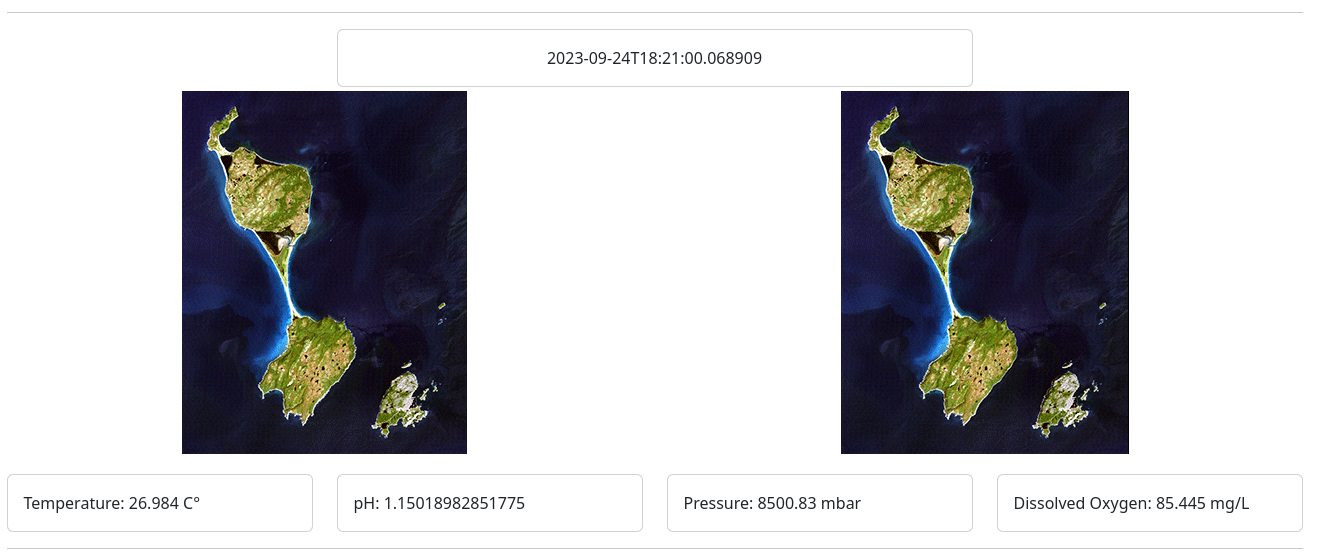
\includegraphics[height=0.65\textheight]{./Figures/study_media_capture_images.png}
		\caption{Media Entry Metadata Page}
	\end{figure}
\end{frame}
\subsection{Study Profile Creation}
\begin{frame}{Study Profile Creation}
	\begin{figure}
		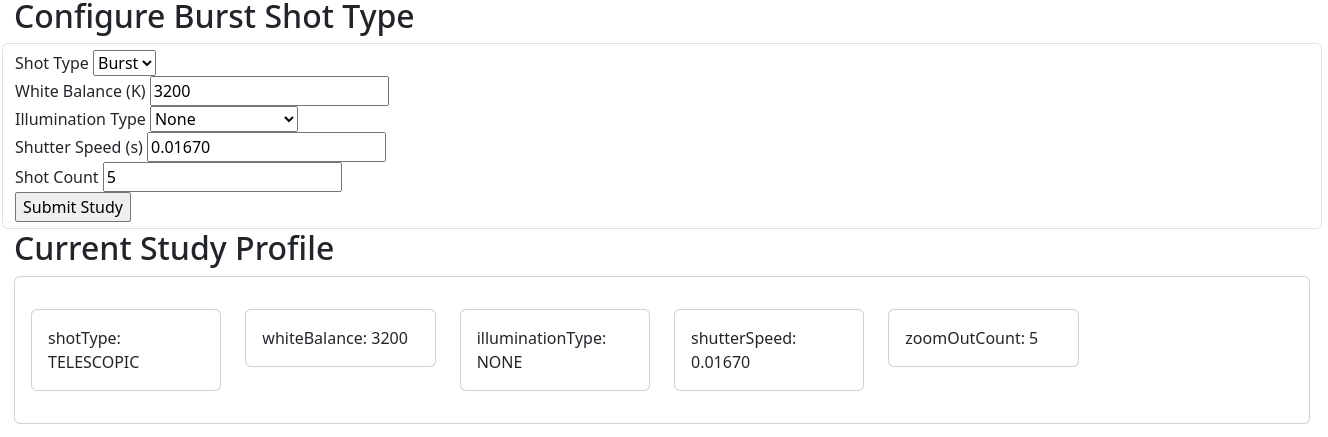
\includegraphics[height=0.60\textheight]{./Figures/study_profile_creation.png}
		\caption{Study Profile Creation Form}
	\end{figure}
\end{frame}
\subsection{Entry Filtering}
\begin{frame}{Entry Filtering: Form}
	\begin{figure}
		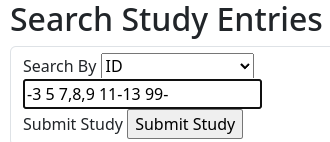
\includegraphics[height=0.55\textheight]{./Figures/entry_filtering_form.png}
		\caption{Media Entry Filtering Form}
	\end{figure}

\end{frame}
\begin{frame}{Entry Filtering: Results}
	\begin{figure}
		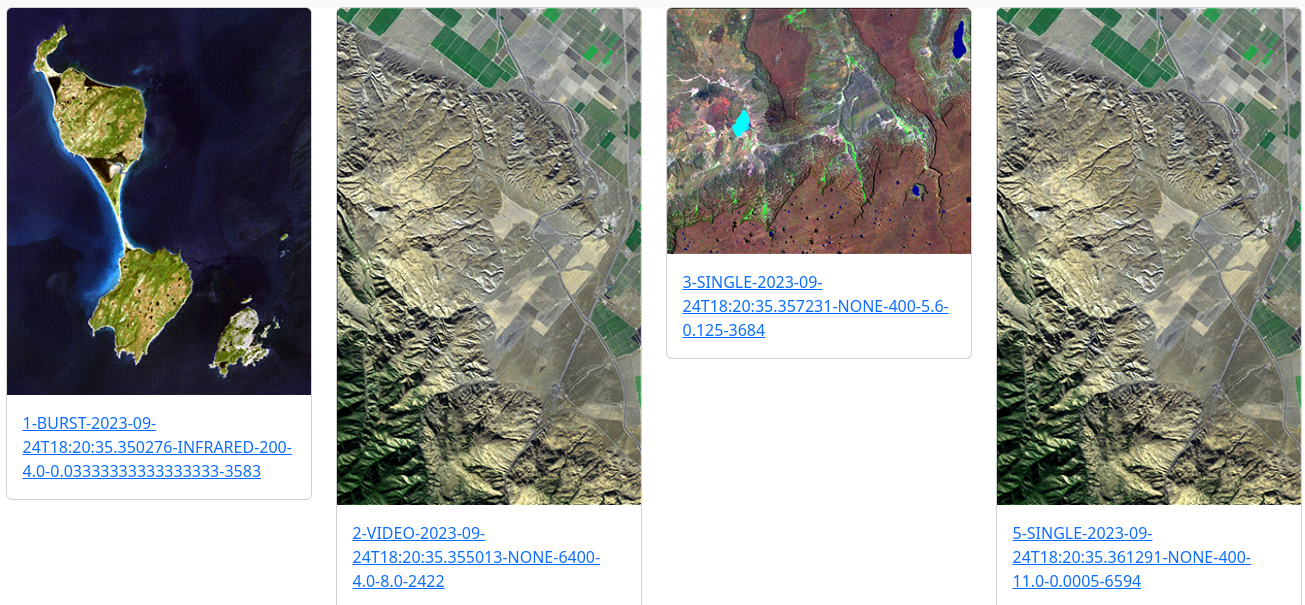
\includegraphics[height=0.55\textheight]{./Figures/entry_filtering_results.png}
		\caption{Media Entry Filtering Results}
	\end{figure}

\end{frame}
\subsection{Automated Raspberry Pi Backup}
\begin{frame}{Automated Microscope Backup}
	\begin{figure}
		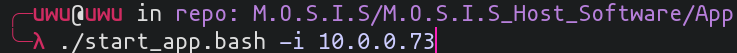
\includegraphics[width=\textwidth]{./Figures/automated_media_backup.png}
		\caption{Start App Command Line Arguments}
	\end{figure}
\end{frame}
\section{Live Demonstration}
\begin{frame}
	\centering Live Demonstration
\end{frame}
\section*{Questions}
\begin{frame}
	\centering Questions?
\end{frame}
\end{document}